% simple document template
\documentclass[dvisvgm]{minimal}
% \documentclass{paper}
\usepackage{tikz}
\usetikzlibrary{graphs}
\usetikzlibrary {mindmap}
\usetikzlibrary {positioning}
\usetikzlibrary {arrows.meta}
\usetikzlibrary {shapes.multipart}
\usetikzlibrary {shapes.geometric}
\usetikzlibrary {shapes.symbols}
\usetikzlibrary {shapes.callouts}
\usetikzlibrary {calc}
\begin{document}

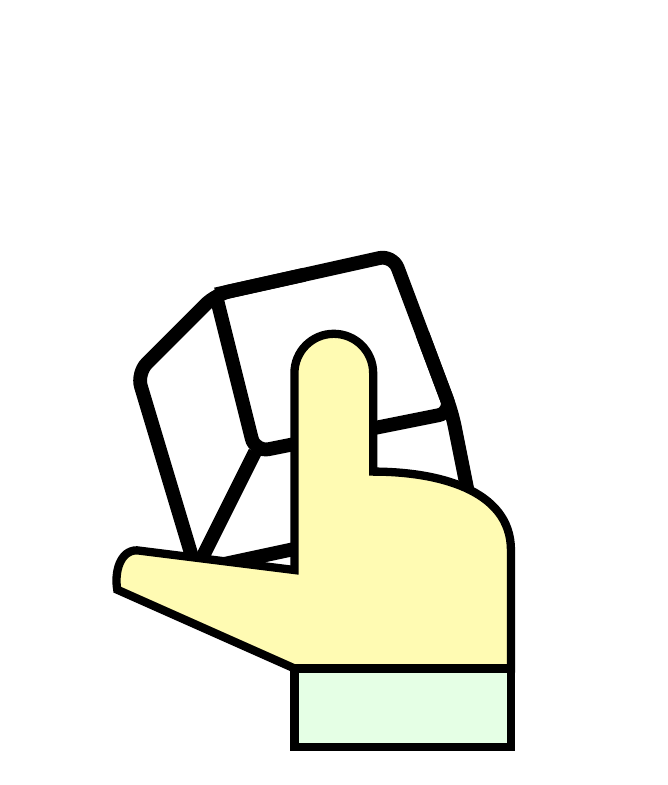
\begin{tikzpicture}[none/.style={}, 
      caps/.style={draw=black, line width=5, rounded corners=5},
      finger/.style={line width=3, fill=yellow!30!white},
      collar/.style={line width=3, fill=green!10!white}
    ]
    % finger
    \node [style=none] (8) at (-0.5, 1.25) {};
    \node [style=none] (7) at (0, 1.75) {};
    \node [style=none] (9) at (0.5, 1.25) {};
    \node [style=none] (10) at (-0.5, -1.25) {};
    \node [style=none] (11) at (-2.5, -1) {};
    \node [style=none] (12) at (-2.75, -1.5) {};
    \node [style=none] (13) at (-0.5, -2.5) {};
    \node [style=none] (14) at (2.25, -2.5) {};
    \node [style=none] (15) at (2.25, -1) {};
    \node [style=none] (16) at (0.5, 0) {};
    \node [style=none] (17) at (-0.5, -3.5) {};
    \node [style=none] (18) at (2.25, -3.5) {};
    % target circle
    \draw[draw=none, fill=white] (7.center) circle (3.5cm);
    \draw[draw=white, line width=5] (7.center) circle (3.8cm);


    \node [none] (0) at (-1.5, 2.25) {};
    \node [none] (1) at (0.75, 2.75) {};
    \node [none] (2) at (-1, 0.25) {};
    \node [none] (3) at (1.5, 0.75) {};
    \node [none] (4) at (-2.5, 1.25) {};
    \node [none] (5) at (-1.75, -1.25) {};
    \node [none] (6) at (1.75, -0.5) {};
    \coordinate (a0) at ($(0.center)!0.5!(1.center)$);
    \coordinate (a1) at ($(1.center)!0.5!(3.center)$);
    \draw[caps] (0.center) to (1.center) to (3.center) to (2.center) to (0.center);
    \draw[caps] (a0) to (0.center) to (4.center) to (5.center) to (6.center) to (3.center) to (a1);
    \draw[caps] (2.center) to (5.center);

    % index finger
    \draw[finger] (8.center) to[in=180, out=90] (7.center) to[in=90, out=0] (9.center) to (16.center)
        to[in=90, out=0] (15.center) to (14.center)
        to (13.center)
        to (12.center)
        to[in=180, out=100] (11.center)
        to (10.center) -- cycle;
    \draw[collar] (13.center) to (17.center) -- (18.center) -- (14.center) -- cycle;

\end{tikzpicture}

\end{document}